\begin{frame}[allowframebreaks]{Cascaded Diffusion Models}
    \begin{figure}
        \centering
        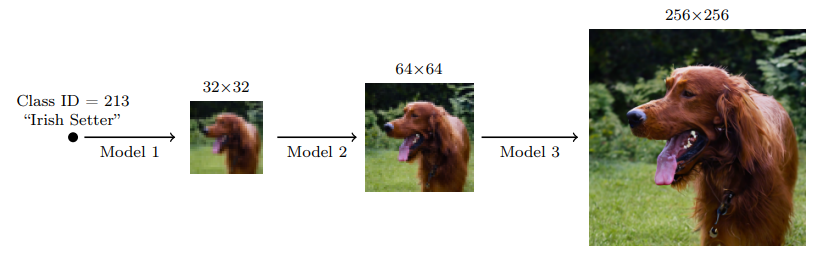
\includegraphics[width=1.06\linewidth,height=\textheight,keepaspectratio]{images/adv-img-gen/slide_102_1_img.png}
    \end{figure}
    \begin{figure}
        \centering
        
\includegraphics[width=0.8\linewidth,height=\textheight,keepaspectratio]{images/adv-img-gen/slide_102_2_img.png}
        \caption*{Ho, Jonathan, et al. "Cascaded diffusion models for high fidelity image generation." The Journal of Machine Learning Research 23.1 (2022): 2249-2281.}
    \end{figure}

    \framebreak

    \begin{itemize}
        \item Train one unconditional model; the remaining models are low-resolution conditional super-resolution models.
        \item Condition on the low-resolution image, perform bilinear or bicubic upsampling, and concatenate the result to the noised input.
        \item Models can be trained independently.
        \item Hyperparameters can be tuned specifically for each resolution.
    \end{itemize}

    \framebreak

    Conditioning Augmentation: Augment the low-res input $z$
    \begin{itemize}
        \item Method 1: Blurring
        \begin{itemize}
            \item Apply a Gaussian blurring filter
            \item Effective for models at 128, 256 resolution
        \end{itemize}
        \item Method 2: Non-truncated Conditioning Augmentation
        \begin{itemize}
            \item Train the super-resolution $p(x|z_0)$ model conditioned on samples from the prior $p(z_0)$ with added corruption from the forward process $q(z_s|z_0)$
            \item $S$ (corruption / noise strength) is a hyperparameter
            \item Effective for resolutions $< 128$
        \end{itemize}
    \end{itemize}

    \framebreak
    \begin{figure}
        \centering
        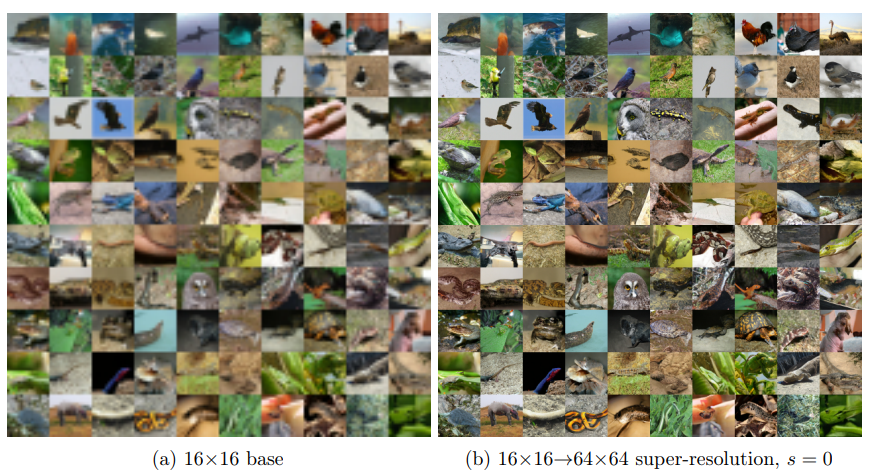
\includegraphics[width=1.06\linewidth,height=0.95\textheight,keepaspectratio]{images/adv-img-gen/slide_105_1_img.png}
    \end{figure}

    \framebreak
    Large improvements in using conditioning augmentation

    \begin{figure}
        \centering
        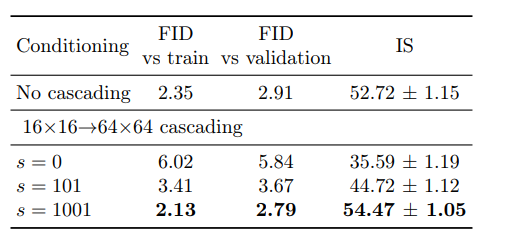
\includegraphics[width=1.06\linewidth,height=0.65\textheight,keepaspectratio]{images/adv-img-gen/slide_106_1_img.png}
    \end{figure}
    
\end{frame}